
\documentclass[acmlarge,nonacm=true]{acmart}
\usepackage{adjustbox}
\usepackage{multirow}
\usepackage{graphicx}
\usepackage{afterpage}
\usepackage{subcaption}

\newcommand\blankpage{%
	\null
	\thispagestyle{empty}%
	\addtocounter{page}{-1}%
	\newpage}

%%
%% \BibTeX command to typeset BibTeX logo in the docs
\AtBeginDocument{%
  \providecommand\BibTeX{{%
    \normalfont B\kern-0.5em{\scshape i\kern-0.25em b}\kern-0.8em\TeX}}}


\begin{document}
	
	\begin{titlepage}
		\begin{center}
			\vspace*{1cm}
			
\includegraphics[width=0.7\textwidth]{fig/ntu_logo}
			\vspace{0.8cm}
			\linebreak
			\Huge
			\textbf{Experiment 4: Implicit Surfaces and Solids}
			
			\vspace{0.5cm}
			\LARGE
			CZ2003 Computer Graphics and Visualization
			
			\vspace{1.5cm}
			\textbf{SS3}\\
			
			\begin{table}[h]
				\begin{tabular}{lc}
					Name & Matric Number \\\hline
					Pang Yu Shao & U17216\underline{\textbf{80}}D \\
				\end{tabular}
			\end{table}
			
			
			
			\vfill
			
			\vspace{0.8cm}
			
			
			
			\Large
			SCHOOL OF COMPUTER SCIENCE AND ENGINEERING\\
			NANYANG TECHNOLOGICAL UNIVERSITY\\
			SINGAPORE\\
			23rd March 2021
			
		\end{center}
	\end{titlepage}

 

%%
%% The "title" command has an optional parameter,
%% allowing the author to define a "short title" to be used in page headers.
\title{CZ2003 Computer Graphics and Visualization}

%%
%% The "author" command and its associated commands are used to define
%% the authors and their affiliations.
%% Of note is the shared affiliation of the first two authors, and the
%% "authornote" and "authornotemark" commands
%% used to denote shared contribution to the research.


\author{Pang Yu Shao}
\email{C170134@e.ntu.edu.sg}
\affiliation{\institution{Nanyang Technological University}}

%%
%% By default, the full list of authors will be used in the page
%% headers. Often, this list is too long, and will overlap
%% other information printed in the page headers. This command allows
%% the author to define a more concise list
%% of authors' names for this purpose.
\renewcommand{\shortauthors}{Pang Yu Shao}






%%
%% This command processes the author and affiliation and title
%% information and builds the first part of the formatted document.

% \begin{teaserfigure}
% 	\includegraphics[width=\textwidth]{bccell}
% 	\caption{Breast Cancer Cell. Photograph by National Cancer Institute [Public domain], via Wikimedia
% 		Commons. (\url{https://w.wiki/kS3}).}
% 	\Description{A breast cancer cell seen through an electron microscope.}
% \end{teaserfigure}
% \maketitle



\tableofcontents
\newpage
\section{Defining Surfaces Implicitly}
\subsection{Plane passing through three defined co-ordinates}
For this exercise, a plane has to be defined such that it passes through three points: 
$(N,M,0)$, $(0,M,N)$ and $(N,0,M)$\\
Since \(N = 8\) and \(M = 10\), the three points are: $A(8,10,0)$, $B(0,10,8)$ and $C(8,0,10)$.\\\\
The implicit function can be defined by: $f(x,y,z) = a(x-x_0) + b(y-y_0) + c(z-z_0)$\\
To obtain the unknowns $a$, $b$ and $c$, a normal vector perpendicular to the plane has to be obtained.\\\\
$\vec{V_1} = \vec{AB} = <(0-8),\ (10-10),\ (8-0)>$\\
$\vec{V_1} = <-8,\ 0,\ 8>$\\\\
$\vec{V_2} = \vec{AC} = <(8-8),\ (0-10),\ (10-0)>$\\
$\vec{V_2} = <0,\ -10,\ 10>$\\\\
$\vec{V_1}\times\vec{V_2} = <(0*10)-(8*-10),\ (8*0)-(-8*10),\ (-8*-10)-(0*0)>$\\
$\vec{V_1}\times\vec{V_2} = <80,\ 80,\ 80>$\\\\
Therefore, $f(x,y,z) = 80(x-x_0) + 80(y-y_0) + 80(z-z_0)$\\\\
Using point A for $x_0$, $y_0$ and $z_0$,\\
$f(x,y,z) = 80(x-8) + 80(y-10) + 80(z)$\\
Since f(x,y,z) = 0,\\
$f(x,y,z) = x-8 + y-10 + z = 0$\\
$\mathbf{f(x,y,z) = x + y + z -18 = 0}$\\\\

As the plane defines an endless plane the bounding box is defined such that 
the three defined points are minimally contained within it, hence the bounding box is defined as:\\ 
$BB_{pos} = (8/2,\ 10/2,\ 10/2) = (4,\ 5,\ 5)$, $BB_{size} = (8,\ 10,\ 10)$
\begin{figure}[H]
	\begin{subfigure}{.33\textwidth}
	  \centering
	  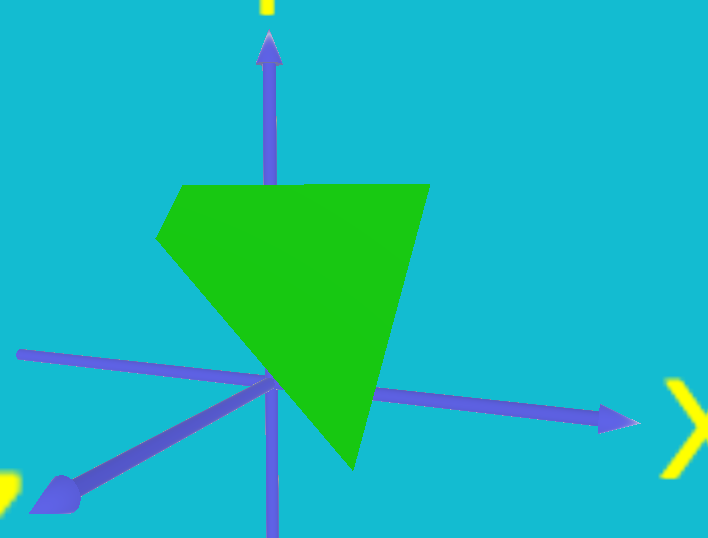
\includegraphics[width=.8\linewidth]{fig/1a1_1_1}
	  \caption{Resolution: 1 1}
	\end{subfigure}%
	\begin{subfigure}{.33\textwidth}
	  \centering
	  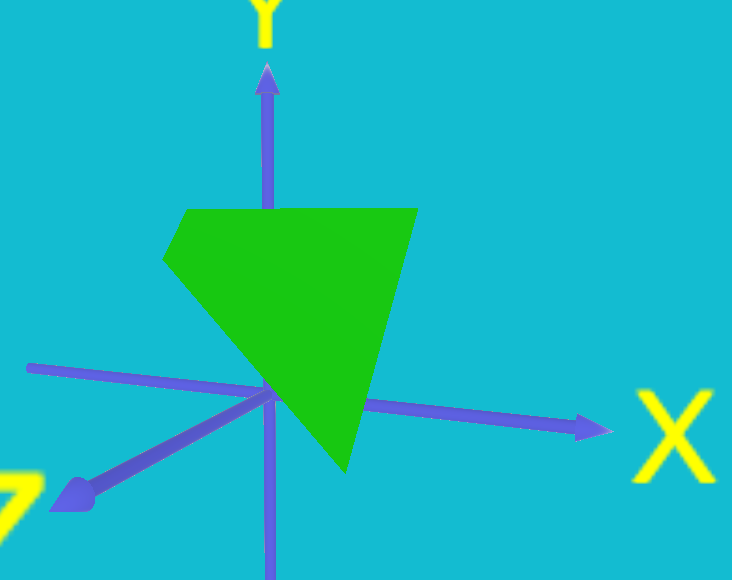
\includegraphics[width=.8\linewidth]{fig/1a10_10_10}
	  \caption{Resolution: 10 10}
	\end{subfigure}
	\begin{subfigure}{.33\textwidth}
		\centering
		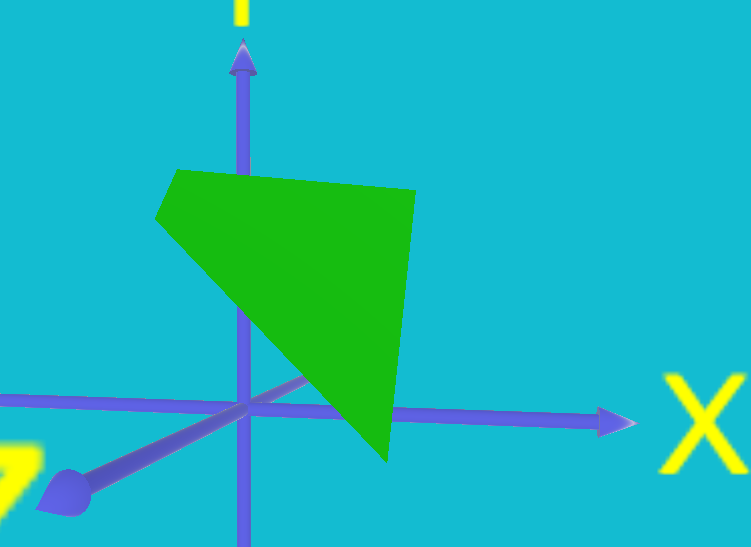
\includegraphics[width=.8\linewidth]{fig/1a100_100_100}
		\caption{Resolution: 1000 1000}
	  \end{subfigure}
	\caption{Plots of the Plane defined in "\textbf{1a.Func}" with differing resolutions}
	\label{fig:1a}
\end{figure}
As seen in Fig. \ref{fig:1a} above, a sampling resolution of \textbf{1} for x,y and z is 
sufficient for rendering the plane and utilizing a higher resolution would
produce the exact same rendering.

\subsection{Half-sphere with defined radius}
To define the lower half of a sphere, we first define a full sphere.
A sphere of radius 10 can be defined with the following implicit function:\\\\
$10^2 - x - y - z \geq 0$\\\\

To obtain a half sphere, a bounding box is defined to only render the bottom half 
of the sphere. Therefore, the bounding box is defined to be centered at: $BB_{pos} = (0,\ 0,\ -5)$\\
Bounding box size: $BB_{size} = (20,\ 20,\ 10)$\\\\
By plotting the implicit function on Shape Explorer with varying resolutions, the following figures were obtained:
\begin{figure}[H]
	\begin{subfigure}{.33\textwidth}
		\centering
		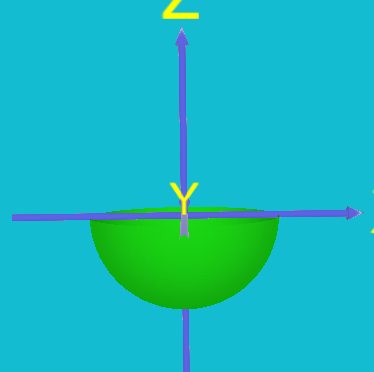
\includegraphics[width=.8\linewidth]{fig/1b50_50_25}
		\caption{Resolution: 50 50 25}
	  \end{subfigure}
	\begin{subfigure}{.33\textwidth}
	  \centering
	  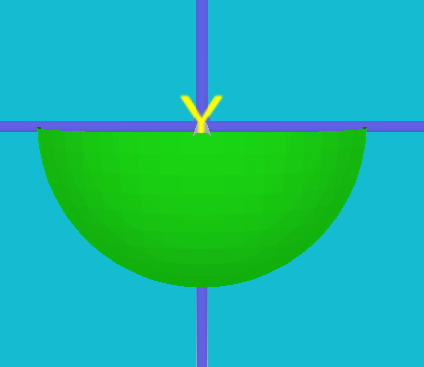
\includegraphics[width=.8\linewidth]{fig/1b20_20_10}
	  \caption{Resolution: 20 20 10}
	\end{subfigure}%
	\begin{subfigure}{.33\textwidth}
		\centering
		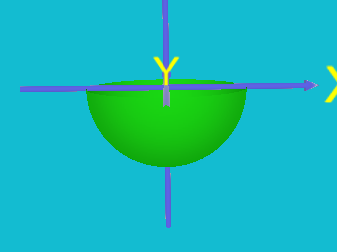
\includegraphics[width=.8\linewidth]{fig/1b100_100_50}
		\caption{Resolution: 100 100 50}
	  \end{subfigure}
	\caption{Plots of the Half-Sphere defined in "\textbf{1b.Func}" with differing resolutions}
	\label{fig:1b}
\end{figure}

As seen in Fig. \ref{fig:1b} above, a sampling resolution of \textbf{50, 50, 25} for x, y and z respectively is optimal 
resolution for rendering the half-sphere. When the resolution is reduced to 20, 20, 10, the surface of the half-sphere is 
not smooth and the polygons that make up the surface can be seen. When the resolution is increased to 100, 100, 50, there 
is no visible difference in the rendered object. However, the rendering time is significantly increased.

\newpage
\subsection{Cylindrical surface with defined height and radius}
\label{section:1c}
To define the a cylindrical surface implicitly, we first define a circle implicitly.
A circle of radius 10 can be defined on the x-y plane with the following implicit function:\\
$10^2 - x - y \geq 0$\\\\

The above implicit function defines a cylindrical surface for the entire Z-axis. Therefore, to render 
it such that it only spans from Z=-8 to Z=10, the bounding box can be defined to be centered at: 
$BB_{pos} = (0,\ 0,\ -1)$\\
Bounding box size: $BB_{size} = (20,\ 20,\ 18)$\\\\ 

By plotting the implicit function on Shape Explorer with varying resolutions, the following figures were obtained:
\begin{figure}[H]
	\begin{subfigure}{.33\textwidth}
	  \centering
	  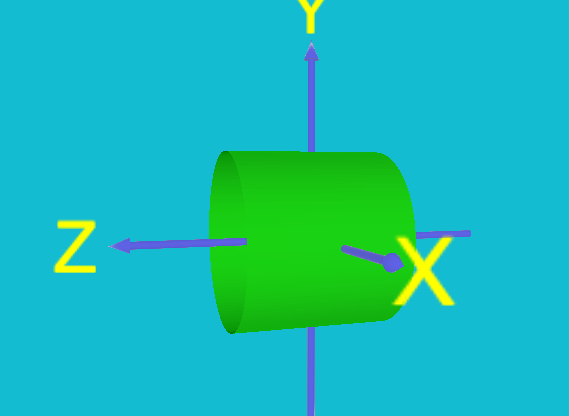
\includegraphics[width=.8\linewidth]{fig/1c50_50_1}
	  \caption{Resolution: 50 50 1}
	\end{subfigure}%
	\begin{subfigure}{.33\textwidth}
	  \centering
	  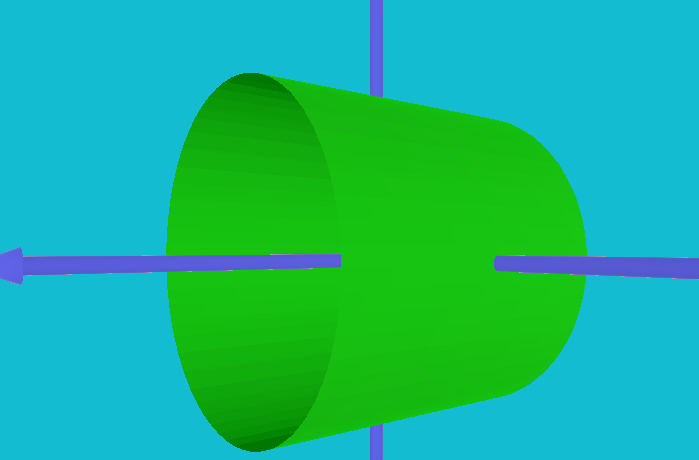
\includegraphics[width=.8\linewidth]{fig/1c20_20_1}
	  \caption{Resolution: 20 20 1}
	\end{subfigure}
	\begin{subfigure}{.33\textwidth}
		\centering
		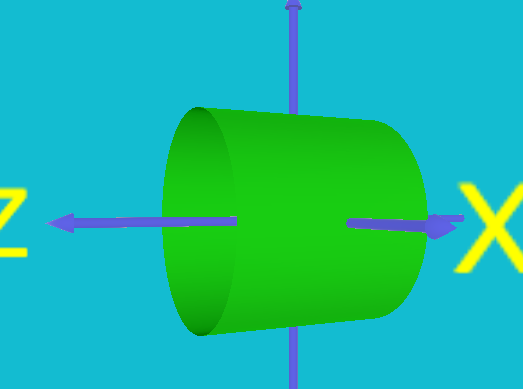
\includegraphics[width=.8\linewidth]{fig/1c100_100_1}
		\caption{Resolution: 100 100 1}
	  \end{subfigure}
	\caption{Plots of the Cylindrical Surface defined in "\textbf{1c.Func}" with differing resolutions}
	\label{fig:1c}
\end{figure}
As seen in Fig. \ref{fig:1c} above, a sampling resolution of \textbf{50, 50, 1} for x, y and z respectively is optimal 
resolution for rendering the cylindrical surface. As the shape does not have any curvature along the z-axis, a resolution 
of 1 is sufficient for the z-axis.

When the resolution is reduced to 20 for both x and y,  the surface of the cylinder is 
not smooth and the interpolations could be seen. When the resolution is increased to 100 for x and y there 
is no observable difference in the rendered object than that when the resolution is 50.

\newpage
\subsection{Two-side conical surface with defined radius and height}
\label{section:1d}
A cone can be defined using the following implicit function:\\
$(x^2 + y^2)/(c^2) - z^2 \geq 0$, where $c = r/h$, which is the ratio of radius to height at some distance from the vertex.\\
Since the cone needs to have a radius of 8(M) at distance 1 from its apex, $c = 8$.\\\\
Therefore, the implicit function to define the cone is:\\
$(x^2 + y^2)/64 - z^2 \geq 0$\\
To render the cone such that it spans from $Z=-1$ to $Z=1$, the bounding box can be defined to be centered at the origin
, $BB_{pos} = (0,\ 0,\ 0)$ with a bounding box size: $BB_{size} = (16,\ 16,\ 2)$\\\\ 

By plotting the implicit function on Shape Explorer with varying resolutions, the following figures were obtained:
\begin{figure}[H]
	\begin{subfigure}{.33\textwidth}
	  \centering
	  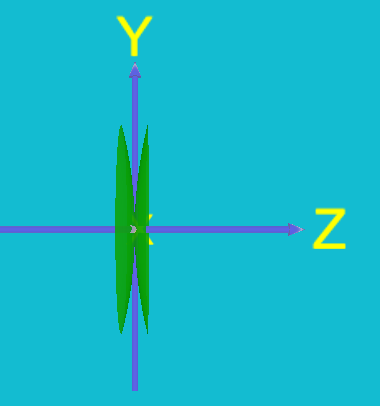
\includegraphics[width=.8\linewidth]{fig/1d40_40_2.PNG}
	  \caption{Resolution: 40 40 2}
	\end{subfigure}%
	\begin{subfigure}{.33\textwidth}
	  \centering
	  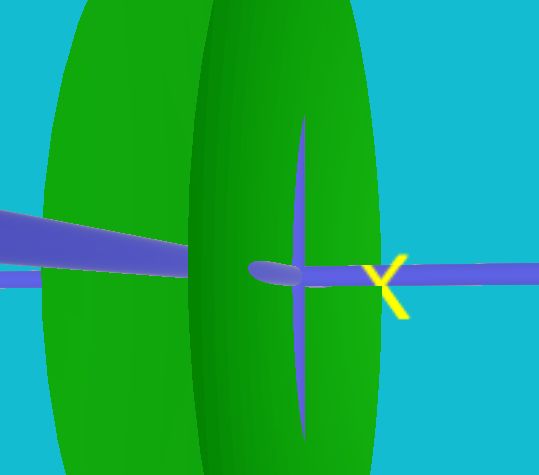
\includegraphics[width=.8\linewidth]{fig/1d20_20_2.PNG}
	  \caption{Resolution: 20 20 2}
	\end{subfigure}
	\begin{subfigure}{.33\textwidth}
		\centering
		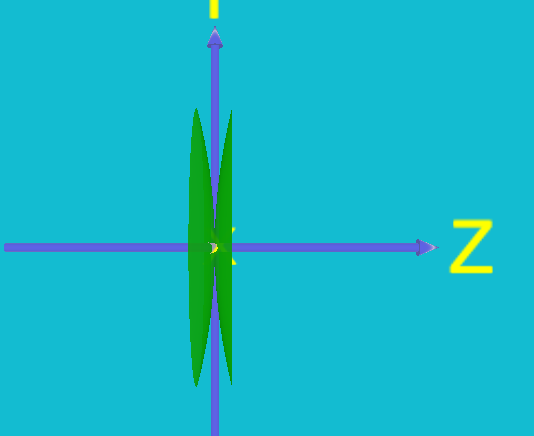
\includegraphics[width=.8\linewidth]{fig/1d100_100_2.PNG}
		\caption{Resolution: 100 100 2}
	  \end{subfigure}
	\caption{Plots of the two-sided cone defined in "\textbf{1d.Func}" with differing resolutions}
	\label{fig:1d}
\end{figure}

When experimenting with the resolutions, it was found that a resolution of \textbf{2} for Z is sufficient for rendering the 
cone shape. The best resolution obtained for rendering the shape was \textbf{40} for x and y. When the resolution for x and y
is decreased to 20, the interpolations could be seen on the surface of the cone when zoomed in (as seen in the figure above). When the resolution was 
increased instead to 100, no visible difference could be seen between that and when the resolution was 40.

\pagebreak
\section{Building Complex Shape with set-theoretic operations}
The complex shape that is to be made is the following:\\
\begin{center}
	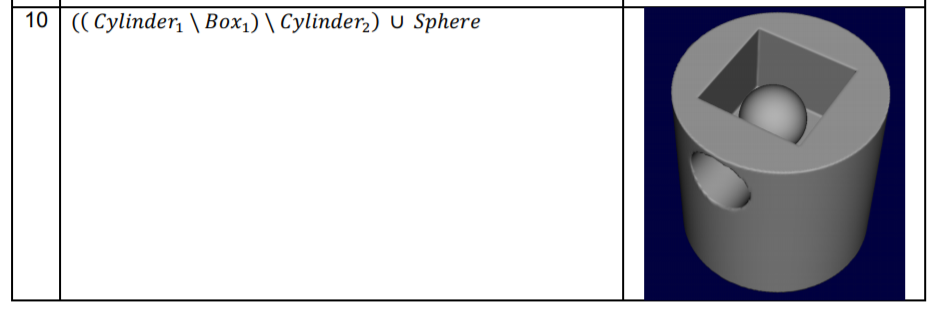
\includegraphics[width = 0.6\textwidth]{fig/2}
\end{center}
Therefore, the following functions are defined to obtain the components of the complex shape:\\\\
$Cylinder_1\mapsto min((5^2 - x^2 - y^2), -z, 10+z)$\\
$Box_1\mapsto min(3-x, x+3, 3-y, y+3, -z, 6+z)$\\
$Cylinder_2\mapsto min((2.5^2 - y^2 - (z+3)^2), -x, 5+x)$\\
$Sphere \mapsto 1.5^2 - x^2 - y^2 - (z+3)^2$\\\\
Thus, the complex shape can be defined with:\\
$Shape \mapsto max(min(min(Cylinder_1, -Box_1), -Cylinder_2)Sphere)$\\\\

To render this complex shape, the bounding box size and position is set to wrap tightly 
over the outer and and larger cylinder: $BB_{pos} = (0,\ 0,\ -5)$, $BB_{size} = (10,\ 10,\ 10)$\\\\

By rendering the shape in Shape Explorer and by varying the resolution, the following 
figures were obtained:\\
\begin{figure}[H]
	\begin{subfigure}{.33\textwidth}
	  \centering
	  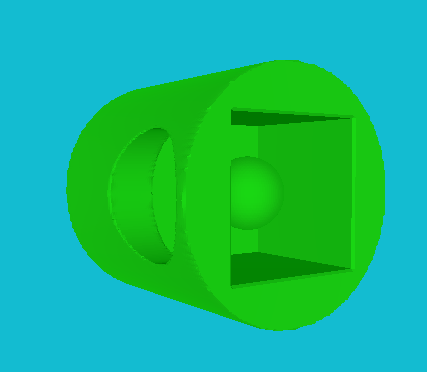
\includegraphics[width=.8\linewidth]{fig/2_100_100_100}
	  \caption{Resolution: 100 100 100}
	\end{subfigure}%
	\begin{subfigure}{.33\textwidth}
	  \centering
	  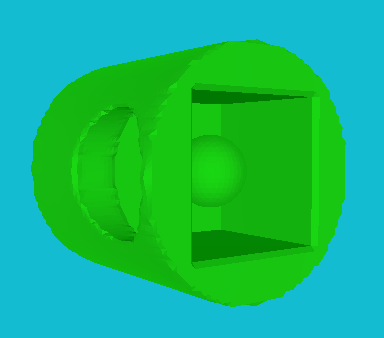
\includegraphics[width=.8\linewidth]{fig/2_50_50_50}
	  \caption{Resolution: 50 50 50}
	\end{subfigure}
	\begin{subfigure}{.33\textwidth}
		\centering
		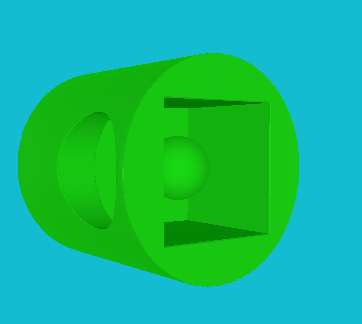
\includegraphics[width=.8\linewidth]{fig/2_200_200_200}
		\caption{Resolution: 200 200 200}
	  \end{subfigure}
	\caption{Plots of the Solid defined in "\textbf{2.Func}" with differing resolutions}
	\label{fig:2}
\end{figure}

The sampling resolution for x, y and z was chosen to be \textbf{100} as it was able to render the shape without the 
polyline interpolations being obvious. When the sampling resolution was reduced to 50, these interpolations are visible 
when zoomed in. If the sampling resolution is increased to 200, there is no visible difference between the original figure 
which was rendered with a resolution of 100.

\section{Colouring Shape with an implicit colour function.}
For this exercise, the tanh function was applied to the colouring function. After scaling the 
function properly such that the values displayed is located within [0,1], the following function
was obtained: $r=tanh((u+5)/10)$.

The bounding box size was increased slightly to (10, 10, 10.2) due to some rendering artifacts
that was only encountered in FVRML.

The following coloured object was obtained.

\begin{figure}[H]
	\begin{subfigure}{\textwidth}
	  \centering
	  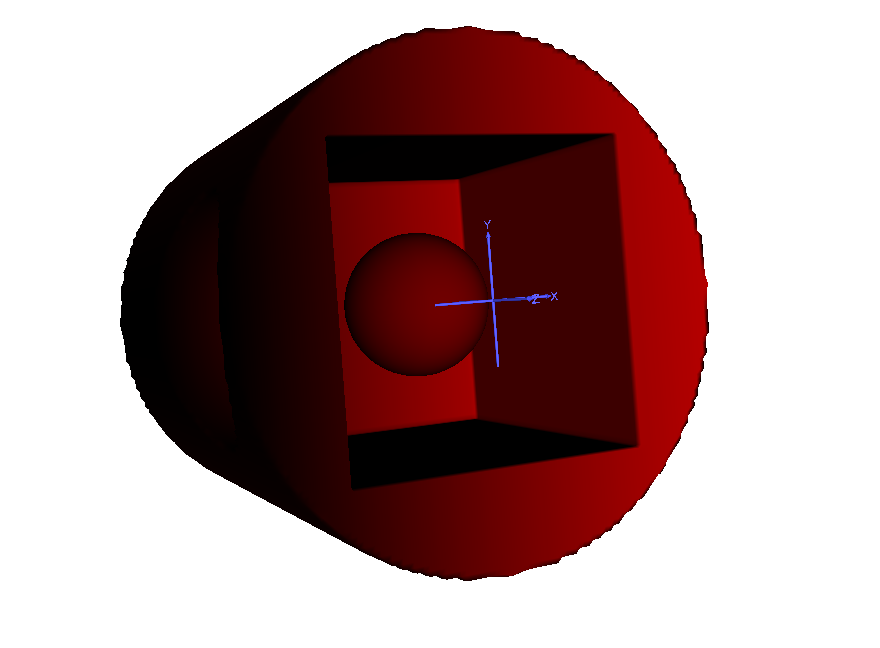
\includegraphics[width=.6\linewidth]{fig/3}
	  \caption{Resolution: 100 100 100}
	\end{subfigure}%
	\caption{Rendering of the coloured Solid defined in "\textbf{3.wrl}"}
	\label{fig:3}
\end{figure}

As the shape is the exact same as the one done in exercise 2, the best sampling resolution would be the same.
Therefore a sampling resolution of \textbf{100, 100, 100} for x, y and z respectively was chosen.


\bibliographystyle{ACM-Reference-Format}
\newpage






\end{document}
\endinput
%%
%% End of file `sample-acmlarge.tex'.
